
\documentclass[a4paper,11pt]{article}

\usepackage{fontspec}
\setmainfont{Calibri}

\linespread{1}

\setlength{\oddsidemargin}{0cm}
\setlength{\evensidemargin}{0cm}
\setlength{\textheight}{23cm}
\setlength{\textwidth}{16cm}

\usepackage{amssymb,mathrsfs,algorithmic,algorithm,multirow, wrapfig}
\usepackage{amsmath,amsbsy,graphicx,color,url,natbib}
\usepackage{ccaption}
\setlength{\bibsep}{0.0pt}


\newcommand{\bm}{\mathbf}
\newcommand{\bs}{\boldsymbol}
\newcommand{\mt}{\mathrm}
\newcommand{\nind}{\noindent}

\usepackage{fancyhdr}
\newcommand{\tstamp}{\today}   
\lhead[\fancyplain{}{\rightmark}]       {\fancyplain{}{}}
\rhead[\fancyplain{}{\rightmark}]       {\fancyplain{}{}}
\chead[\fancyplain{}{\centermark}]       {\fancyplain{}{ENGM214 -- Process Modelling and Simulation} }
\pagestyle{fancyplain}

\usepackage{amsthm}
\theoremstyle{definition}
\newtheorem{exmp}{Example}[section]

\title{\vspace{-2cm} Lecture 5 -- Solution strategies for lumped parameter systems}

\author{Tao Chen\\
{\small \emph{Department of Chemical \& Process Engineering, University of Surrey, UK}}\\
{\small (email: \texttt{t.chen@surrey.ac.uk}; \hspace{0.5cm} updated on: \today )}
}
\date{}

\begin{document}
\maketitle

%\tableofcontents
\vspace{-0.5cm}

\section{Solving algebraic equations -- a quick review}
\label{sec:alg}

The topic of \emph{linear algebra} deals with systems of linear equations.

\begin{exmp}[A separation system]
\label{exmp:separ}
A simple example was discussed in Tutorial 1 where we tried to find the mass flow rates $x_1$,
$x_2$ and $x_3$.

\begin{figure}[!h]
 \begin{center}
	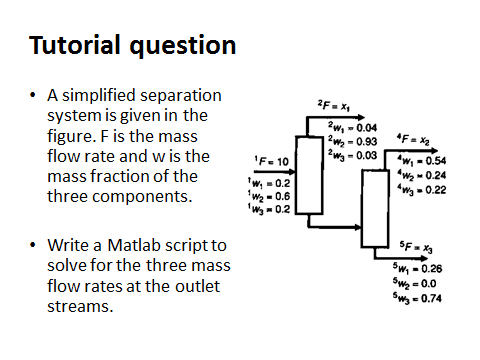
\includegraphics[width=.5\textwidth]{separ}
 \end{center}
 \caption{Tutorial 1 slide.} 
 \label{fig:separ}
\end{figure}


The mathematical model for this steady-state system was due to conservation of mass.
By defining the combination of the two vessels as our balance volume,
we have

\begin{align}
	x_1 + x_2 + x_3 &= 10 \\
	0.04 x_1 + 0.54 x_2 + 0.26 x_3 &= 2 \\
	0.93 x_1 + 0.24 x_2 + 0.0 x_3  &= 6
\end{align}

\end{exmp}

In general, through modelling we may obtain a linear system with $m$ linear equations with $n$ unknowns
($x_1, \ldots, x_n$):
\begin{align}
	a_{11} x_1 &+ a_{12} x_2 + \cdots + 	a_{1n} x_n = b_1 \\
	a_{21} x_1 &+ a_{22} x_2 + \cdots + 	a_{2n} x_n = b_2 \\	
	                 &\vdots \\
	a_{m1} x_1 &+ a_{m2} x_2 + \cdots + 	a_{mn} x_n = b_m
\end{align}
\noindent By introducing vector-matrix form, this linear system is:
\begin{equation}
	\bm{A x} = \bm b
\end{equation}
\noindent where $\bm A$ is an $m \times n$ matrix, $\bm x$ is a column vector with $n$ entries, and $\bm b$ is a column
vector with $m$ entries:

\begin{equation}
	\bm A = \left[ 
		\begin{array}{cccc}
			a_{11} & a_{12} & \cdots & a_{1n} \\
			a_{21} & a_{22} & \cdots & a_{2n} \\
			\vdots  & \vdots   & \ddots & \vdots \\
			a_{m1} & a_{m2} & \cdots & a_{mn}
		\end{array} \right], \quad
	\bm x = \left[
		\begin{array}{c}
			x_1 \\
			x_2 \\
			\vdots \\
			x_n
		\end{array} \right], \quad
	\bm b = \left[
		\begin{array}{c}
			b_1 \\
			b_2 \\
			\vdots \\
			b_m
		\end{array} \right]
\end{equation}
\noindent The classical method to solve this linear system is ``Gaussian elimination'';
refer to \url{https://en.wikipedia.org/wiki/Gaussian_elimination} for how it works.

If the algebraic equations are \textbf{non-linear} with respect to $\bm x$, solution methods become more
complicated. In Tutorial 2, we examined how to use Matlab built-in function \texttt{fsolve} to solve general
non-linear algebraic equations. 

The most widely used method for solving a non-linear algebraic equation,
$f(x) = 0$, is the \textbf{Newton-Raphson} method. It works be starting from an initial guess of
the solution, say $x_0$, where the subscript denotes ``iteration 0'', and then iterates from
iteration $n$ to $n+1$ until convergence as follows:

\begin{equation}
	x_{n+1} = x_n - \frac{f(x_n)}{f'(x_n)}
\end{equation}
\noindent where $f'(x_n)$ is the derivative of $f$ with respect to $x$ and evaluated at $x_n$.

For systems of non-linear algebraic equations, $\bm f(\bm x)=\bm 0$, the Newton-Raphson method
can be adapted accordingly to find the solution. Note that the question at the end of Tutorial 2 is an example
of a system of two non-linear algebraic equations.
Readers are referred to \url{https://en.wikipedia.org/wiki/Newton\%27s_method} for
more detailed description of the Newton-Raphson method. There are also other methods
for solving non-linear algebraic equations, such as the secant method and the bisection
method. Readers are encouraged to Google these methods for a quick review.


\section{Solving odinary differential equations (ODEs)}

The basic concept of solving differential equations (both ODEs and partial differential equations (PDEs)),
using \emph{numerical methods}, is to \textbf{discretise}. That is, we discretise the continuous independent
variables (time and space) into discrete ``points'' in time and space, and then seek to find the
solution at these points. Fig. \ref{fig:solver_clas} gives the categories of ODE solvers.

\begin{figure} [!h]
 \begin{center}
	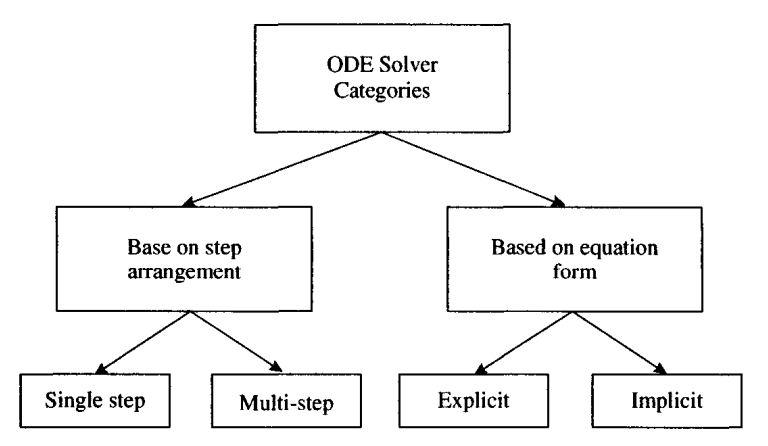
\includegraphics[width=.6\textwidth]{solver_class}\\
 \end{center}
 \caption{Categories of ODE solvers.} 
 \label{fig:solver_clas}
\end{figure}

\subsection{The basic methods}

The methods discussed here apply to the case of a single variable (i.e. a scalar $x$)
as well as multiple variables (i.e. a vector $\bm x$).

\subsubsection*{The Euler's method}

Let's start with the simplest method for solving ODEs: the \textbf{Euler's} method. For a general
ODE, $dx / dt = f(x, t)$ with given initial condition $x(t=0)$, suppose we seek to find solution of $x$
at chosen time points $t_0, t_1, \ldots, t_n$. The \emph{single-step explicit Euler's method} works
by the so-called \textbf{finite difference method} to approximate differentiation. 
For example when advancing from $t_0$ to $t_1$, we have
\begin{equation}
	\frac{d x}{d t}\Big|_{t=t_0} \approx \frac{ x(t_1) - x(t_0) }{t_1 - t_0} = \frac{ \textrm{change of } x }{ \textrm{change of } t }
\end{equation}
\noindent Since the ODE is $dx / dt=f(x,t)$, the left-hand side of the above
is $(dx / dt)|_{t=t_0} = f(x_0,t_0)$, where we use the notation $x_0 = x(t=t_0)$.
Therefore,
\[
	f(x_0,t_0) \approx \frac{ x_1 - x_0 }{t_1 - t_0}
\]
\noindent which can be re-arranged to give a formula to calculate $x_1$ at $t_1$, when $x_0$ is known at $t_0$ 
($x_0$ must be known since it's the initial condition):
\begin{equation}
	x_1 = x_0 + f(x_0,t_0) (t_1 - t_0)
\end{equation}

Now with $x_1$ calculated, we can repeat the same process to calculate $x_2$ at $t_2$ 
($x_2 = x_1 + f(x_1,t_1) (t_2 - t_1)$, and $x_3$ at $t_3$, and so on,
until the last time point $t_n$. In general, the formula for the single-step explicit Euler's method is
\begin{equation} \label{eq:euler}
	x_n = x_{n-1} + f(x_{n-1}, t_{n-1}) (t_n - t_{n-1})
\end{equation}


\begin{exmp}[Using Euler's method to solve $dx/dt=-0.5 x, x(0) = 100$]
\label{exmp:euler}
In fact, we don't need Euler's method to solve this because it has an exact, analytical
solution of $x(t) = x(0) e^{-0.5 t}$. Nevertheless, with known analytical solution we
can compare how the numerical solution performs, and for more complex ODEs analytical solutions may not exist.

\begin{figure} [!h]
 \begin{center}
	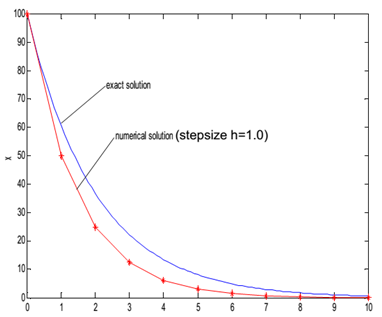
\includegraphics[width=.45\textwidth]{euler}\\
 \end{center}
 \caption{Illustration of solveing $dx/dt=-0.5 x, x(0) = 100$ at $t=0, 1, \ldots, 10$.} 
 \label{fig:euler}
\end{figure}

In this case, $x_0 = 100$, and 
\[ 	x_1 = x_0 + f(x_0,t_0) (t_1 - t_0) = 100 + -0.5 \times 100 \times 1 = 50, \]
and so on.
The results are shown in Fig. \ref{fig:euler}. Note that by taking
equal intervals in time, i.e. $t_1-t_0 = t_2-t_1 = \cdots = t_n - t_{n-1}$,
we normally term this time interval \emph{stepsize} $h = t_1 - t_0$.
Clearly, the numerical solution significantly deviates from the analytical solution.
This is because the stepsize is too big. To see this, we can apply the same Euler's method
with different stepsizes, and the results are ilustrated in Fig. \ref{fig:euler_stepsize}.

\begin{figure} [!h]
 \begin{center}
	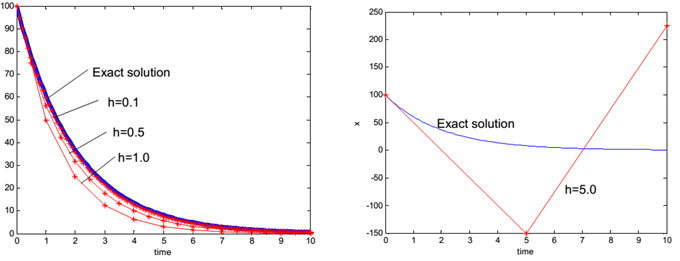
\includegraphics[width=.9\textwidth]{euler_stepsize}\\
 \end{center}
 \caption{The effect of stepsize on Euler's method.} 
 \label{fig:euler_stepsize}
\end{figure}

\end{exmp}

From Fig. \ref{fig:euler_stepsize} some general conclusions can be drawn, which apply to
any numerical methods for solving ODEs:
\begin{itemize}
	\item Smaller stepsizes may improve the accuracy (i.e. reduce error), however at the cost of more computational effort 
		(more steps to go through in order to complete a simulation of a given length of time).
	\item Increasing stepsizes normally reduces the accuracy while accelerating the calculation. However, a too large stepsize may 
		lead to an unstable solution process (Fig. \ref{fig:euler_stepsize}, right panel).
	\item A good numerical solution process should be stable and maintain the right balance between accuracy and efficiency.
		This process is determined by the method applied, the parameter chosen (e.g. the stepsize), and the problem at hand.
\end{itemize}

\subsubsection*{The concept of explicit vs implicit, and single-step vs. multi-step}

The Euler's method discussed above is an explicit method. It provides
an \textbf{explicit} calculation of $x_n$ without solving any equation iteratively
(see eq. (\ref{eq:euler}). Alternatively, we could construct an implicit Euler's method,
by replacing $f(x_{n-1}, t_{n-1})$ with $f(x_n, t_n)$. This is a valid approach and sometimes
called \emph{backward difference} (see \url{https://en.wikipedia.org/wiki/Finite_difference}).
The resulting formula becomes:
\begin{equation} \label{eq:euler_imp}
	x_n = x_{n-1} + f(x_n, t_n) (t_n - t_{n-1})
\end{equation}
\noindent Notice that eq. (\ref{eq:euler_imp}) does not offer an explicit expression for calculating $x_n$,\
\footnote{In some special cases depending on the form of $f(x, t)$, one may re-arrange 
eq. (\ref{eq:euler_imp}) to obtain an explicit expression. However this may not work in general.}
since $x_n$ appears on both sides of the equation. 
But please note that eq. (\ref{eq:euler_imp}) is an algebraic equation, and in general the whole
idea of numerical ODE solution is to turn differential equation(s) into algebraic equation(s).
Therefore, we normally use the numerical methods discussed in Section \ref{sec:alg} to solve this algebraic equation.

In general, the explicit and implicit alternatives exist for many other numerical solution techniques that
are more complex than the Euler’s. We will show later that the implicit methods, although are more complex
and require more computation (because of the iterative method needed to solve the algebraic equation),
have some advantages over the explicit methods.

Both explicit and implicit Euler's methods are of \textbf{single-step}: the calculation involves only one
past step ($n-1$) in order to calculate the current step $n$). In contrast, there are methods which require
the use of the several past steps in order to calculate the current step. Such methods are called 
\textbf{multi-step} methods.

\begin{exmp}[The two-step LMM (Linear Multi-step Method)]
\label{exmp:lmm}
The two-step LMM for solving an ODE $dx / dt = f(x, t)$ with given initial condition $x(t=0)$
is as follows (notice the formulation is from calculating $x_{n+2}$ based on $x$ at the previous two
time steps $x_{n+1}$ and $x_n$:
\begin{equation} \label{eq:lmm}
	x_{n+2} = - ( \alpha_0 x_n + \alpha_1 x_{n+1}) 
		+ h \left( \beta_0 f(x_n) + \beta_1 f(x_{n+1}) + \beta_2 f(x_{n+2}) \right)
\end{equation}
\noindent where $h$ is stepsize, $\alpha$'s and $\beta$'s are coefficients depending on the design of this method.

\end{exmp}

\subsubsection*{Runge-Kutta methods: single-step, explicit or implicit}

The Runge-Kutta (RK) methods are one of the most widely used for solving ODEs. 
For example, the Matlab built-in ODE solver, \texttt{ode45}, is based on an explicit ``RK (4,5)'' formula.
Let's start from re-writing the explicit Euler's method in eq. (\ref{eq:euler}) using a fixed
timestep $h=t_{n+1}-t_n$ when progressing from $t_n$ to $t_{n+1}$:
\begin{equation}
	x_{n+1} = x_n + h f(x_n, t_n)
\end{equation}
\noindent where the key computation relates to the gradient (i.e. the right-hand side of the ODE), 
$f(x_n, t_n)$. The basic idea of RK methods is that, instead of calculating
this gradient in one go (like the Euler's method), it is evaluated at several time points
between $t_n$ and $t_{n+1}$:
\[ f(x_{n,i}, t_{n,i}), \; t_n \leq t_{n,i} \leq t_{n+1}, \; i = 1, \ldots, s \]
Then, a weighted average, $\sum_{i=1}^s b_i f(x_{n,i}, t_{n,i})$ with $b_i$ being the weights, 
replaces a single-point calculation $f(x_n, t_n)$ to give:
\begin{equation} \label{eq:rk_general_1}
	x_{n+1} = x_n + h \sum_{i=1}^s b_i f(x_{n,i}, t_{n,i}) 
\end{equation}
\noindent The above calculation requires $x_{n,i}$, which themselves must be calculated from
time point $t_n$ to these intermediate time points $t_{n,i}$. 
These calculations follow the similar weighted average method as:
\begin{equation} \label{eq:rk_general_2}
	x_{n,i} = x_n + h \sum_{j=1}^s a_{i,j} f(x_{n,j}, t_{n,j}), \; i = 1, \ldots, s 
\end{equation}
\noindent where the time points are
\begin{equation} \label{eq:rk_general_3}
	t_{n,j} = t_n + c_j h
\end{equation}

Eqs. (\ref{eq:rk_general_1})(\ref{eq:rk_general_2})(\ref{eq:rk_general_3}) form the
general formula for the family of RK methods. The number of intermediate ``stages'' is
denoted by $s$, and the parameters, $a_{i,j}, b_i, c_j$, determine what particular
RK method is to be used. 

\textbf{Conditions for an explicit RK method.}
Note that depending on the values of $a_{i,j}$'s, the RK method can be either explicit or implicit.
If $a_{i,j} = 0$ for any $j \geq i$, the resulting RK method is explicit; 
otherwise it is implicit\footnote{Please prove this statement.}.

\textbf{How to determine the RK method's parameters?} The fundamental principle of RK methods
is to match Taylor series of a specific order, which also determines the order the accuracy of a
particular RK method. Note that the number of stages in a RK method (i.e. $s$ in 
eqs. (\ref{eq:rk_general_1})(\ref{eq:rk_general_2})(\ref{eq:rk_general_3})) is not always the same as
the order of accuracy. 

We do not intend to delve into more detailed theories of RK methods; for more information refer to \citep{Brenan1989}.
For details on Matlab implementation of the ODE solvers, see \citep{Shampine1997}.
Below we list the formula for two RK methods.

\begin{exmp}[The explicit midpoint method (a 2-stage 2nd-order RK method)]
\label{exmp:rk_mid}
In this case, $s=2$ (i.e. 2-stage); $a_{11} = a_{12} = a_{22} = 0$, $a_{21}=0.5$;
$b_1=0, b_2=1$; $c_1=0$, $c_2=0.5$. The formulae are:
\begin{equation} \label{eq:rk_mid_1}
	x_{n+1} = x_n + h f( x_{n, 2}, t_n + 0.5 h)
\end{equation}
\noindent where
\begin{equation} \label{eq:rk_mid_2}
	x_{n,2} = x_n + 0.5 h f( x_n, t_n)
\end{equation}
\noindent Starting from $x_n$ at $t_n$, this method first calculates $x_{n,2}$
using eq. (\ref{eq:rk_mid_2}), and then substitute $x_{n,2}$ into eq. (\ref{eq:rk_mid_2})
to calculate $x_{n+1}$.
\end{exmp}

\begin{exmp}[A popular 4th-order RK method (4-stage 4th-order)]
\label{exmp:rk_4}
The formula is
\begin{equation} \label{eq:rk_4}
	x_{n+1} = x_n + \frac{1}{6} h (k_1 + 2 k_2 + 2 k_3 + k_4)
\end{equation}
\noindent where
\begin{align} \label{eq:rk_2}
	k_1 &= f( x_n, t_n) \\
	k_2 &= f( x_n+\frac{1}{2} k_1 h, t_n + \frac{1}{2} h) \\
	k_3 &= f( x_n+\frac{1}{2} k_2 h, t_n + \frac{1}{2} h) \\
	k_4 &= f( x_n+ k_3 h, t_n + h)
\end{align}
\noindent Starting from $x_n$ at $t_n$, this method first calculates $k_1, k_2, k_3, k_4$ as above, 
and then substitute $k$'s into eq. (\ref{eq:rk_4})
to calculate $x_{n+1}$.

\textbf{Verify} that for this RK4 method, the parameters are:
$s=4$; $a_{21} = a_{32} = 1/2, a_{43} = 1$, all other $a$'s are zero;
$b_1=1/6, b_2=b_3=1/3, b_4=1/6$; $c_1=0$, $c_2=c_3=1/2, c_4=1$.

\end{exmp}


\subsubsection*{Backward differentiation formulae (BDF) methods: multi-step, implicit}

A number of linear multi-step methods (LMM, e.g. Adams-Bashforth method, Adams-Moulton method)
can be represented in the following form:
\begin{equation} 
	\sum_{j=0}^k \alpha_j x_{n+j} = h \sum_{j=0}^k \beta_j f ( x_{n+j}, t_{n+j} )
\end{equation}
\noindent These are termed ``linear'' because the formula is in linear form of $x$ (left-hand side of the equation)
\emph{and} of $f ( x_{n+j}, t_{n+j} )$ (right-hand side of the equation); it is not necessarily in linear form of $x$.
Note that when $\beta_k \neq 0$, the methods are implicit because $x_{n+k}$, the latest step to be
calculated, apepars on both sides of the formula.

A special form of the general LMM formula is
\begin{equation} 
	\alpha_0 x_n + \alpha_1 x_{n+1} + \cdots + \alpha_k x_{n+k} = h \beta f ( x_{n+k}, t_{n+k} )
\end{equation}
\noindent which is called a backward differentiation formula, as the derivative, $f ( x_{n+k}, t_{n+k} )$,
at the ($n+k$)-th time point is represented by back (past) values of the solution
($x_{n+k-1}, x_{n+k-2}, \ldots, x_n$). These BDF methods are capable of dealing with ``stiff'' problems and more efficient than 
single-step methods particularly for problems involving complex right-hand sides. They are widely used
in practice for such applications and are the basis of a large number of popular numerical codes.

\subsection{Common issues of ODE systems}
So far we have discussed various types of ODE solution methods.
These methods have different properties in terms of efficiency, stability, and accuracy.
In the following, we discuss these concepts in greater detail, however in a less mathematical manner in order to
help you quickly grasp the main concepts; for more rigorous analysis refer to \citep{Brenan1989, Hangos2001}.

\subsubsection*{Stability of ODE systems}

\begin{exmp}[A linear ODE]
\label{exmp:stab_linear}
Consider a linear ODE
\begin{equation} \label{eq:stab_lin}
	\frac{d y}{d t} = \lambda y, \quad \textrm{with} \quad y(0) = y_0
\end{equation}
\noindent which has an exact solution of $y(t) = y_0 e^{\lambda t}$.
For $\lambda$ that is of real values, and Fig. \ref{fig:stab_lin}
gives the solution for different $\lambda$. Clearly when $\lambda \leq 0$, the system is ``stable'',
or in other words it tends to a finite value when $t \to \infty$.
\begin{figure} [!h]
 \begin{center}
	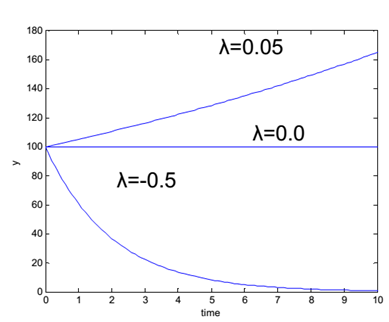
\includegraphics[width=.5\textwidth]{stab_lin}\\
 \end{center}
 \caption{The solution of $dy/dt=\lambda y$ with $\lambda=0.05, 0.0, and -0.5$ and $y_p=100$.} 
 \label{fig:stab_lin}
\end{figure}

If $\lambda$ is a complex number of the form of $a + b j$ where $j=\sqrt{-1}$,
the analytical solution becomes $y(t) = y_0 e^{\lambda t} = y_0 e^{(a+b j) t} = y_0 e^{a t} [ \cos (bt) + j \sin (bt) ] $.
Similarly the solution tends to a finite value when $t \to \infty$, if and only if $a \leq 0$. This means that
the real part of the complex number $\lambda$ must be non-positive, denoted as
$\textrm{Re}(\lambda) \leq 0$.
\end{exmp}

\begin{exmp}[A linear system of ODEs]
\label{exmp:stab_linear_systems}
Now consider multiple ODEs described by
\begin{equation} \label{eq:stab_lin}
	\frac{d \bm y}{d t} = \bm A \bm y + \bm g(t), \quad \textrm{with} \quad \bm y(0) = \bm 0
\end{equation}
\noindent where $\bm y$ is a vector at any time point, $\bm g(t)$ is a vector-valued function that is independent
of $\bm y$. 

\textbf{Question:} what can be said about the stability of the above system?
\textbf{Answer:} Use the eigenvalues of $\bm A$.\footnote{Eigenvalues and eigenvectors are fundamental concept
in linear algebra. If you are not familiar with these, refer to any textbook in engineering mathematics
or \url{https://en.wikipedia.org/wiki/Eigenvalues_and_eigenvectors}. The Matlab built-in function to calculate
the eigenvalues of a matrix is \texttt{eig}.}
Let $\lambda_i, i=1,\ldots, n$ be the eigenvalues of $\bm A$, then this linear system of ODEs is stable if
all eigenvalues have non-positive real part; if any $\lambda_i$ has a positive real part, then the system is unstable.

Note that complex eigenvalues are common. For example, a seemingly simple matrix
\[
	\bm A = \left[ \begin{array}{cc}
		3 & -2 \\
		4 & -1 \\ \end{array} \right]
\]
\noindent has two complex eigenvalues $\lambda = 1\pm 2j$.
\end{exmp}

From the above two examples, what can we deduce about the stability of non-linear systems of ODEs of the following?
\begin{equation}  \label{eq:stab_nonlin}
	\frac{d \bm y}{d t} = \bm f( \bm y, t), \quad \textrm{with} \quad \bm y(0) = \bm y_0
\end{equation}
\noindent The answer is to use the Jacobian matrix, $\bm J$, whose $(i,j)$-th entry is defined as
\begin{equation} 
	J_{i,j} = \left[ \frac{\partial f_i}{\partial y_j} \right]
\end{equation}
\noindent and to calculate the eigenvalues $\lambda_i$ of the Jacobian matrix $\bm J$.
Similar to the above, these eigenvalues can tell the stability of the ODE system.
Notice that $\bm J$ depends on specific values of $\bm y$, and thus the stability also depends on
specific values of $\bm y$. Since $\bm y$ changes with time , which is what ODEs try to describe,
we can only tell the ``local stability'' of the system around the specific values of $\bm y$.

The stability criterion and the eigenvalue-based method are important for the developments in the remaining of this lecture.


\subsubsection*{Stiffness of ODE systems}

We illustrate the issue of stiffness, which does not apply to a single ODE but a system of ODES, 
with the following example.

\begin{exmp}[A stiff ODE system]
\label{exmp:stiff}
Consider the following two-dimensional ODE system $\bm y = [y_1, y_2]'$
\begin{equation} 
	\frac{d \bm y}{d t} = \bm A \bm y + \bs \phi
\end{equation}
\noindent with
\begin{equation}
	\bm A = \left[
		\begin{array}{cc}
			-2000 & 999.75 \\
			1       & -1 \\
		\end{array} \right], \quad
	\bs \phi = \left[
		\begin{array}{c}
			1000.25 \\
			0 \\
		\end{array} \right], \quad
	\bm y(0) = \left[
		\begin{array}{c}
			0 \\
			-2 \\
		\end{array} \right]
\end{equation} 

This is a special case where the analytical solution exists:
\begin{align}
	y_1(t) &= -1.499 e^{-0.5 t} + 0.499 e^{-20005 t} + 1 \\
	y_2(t) &= -2.999 e^{-0.5 t} - 0.0025 e^{-20005 t} + 1 	
\end{align}
Note that in the solution of each state variable, there is a slow transient element ($e^{-0.5 t}$)
and a fast-transient element ($e^{-20005 t}$). After the initial period, the fast-transient element will die out 
and from then on the system’s behaviour is dominated by the slow transient element. Numerically, this fast-transient element 
could control the step size not only for the accuracy of the solution at the early stage but also for the stability throughout the simulation. 
A very small step size will be kept through the entire solution process, hence making a (unnecessarily) very inefficient process (too many solution steps).

\end{exmp}

We call such an ODE system as a ``stiff'' system. In general, this refers to the significance difference in the order of 
magnitude of the \textbf{eigenvalues} of the coefficient matrix $\bm A$ as in the linear ODE system  in eq. (\ref{eq:stab_lin}),
or that of the Jacobian matrix $\bm J$ as in the non-linear ODE ssytem in eq. (\ref{eq:stab_nonlin}). 
Special care is needed for this type of system in order to get the right balance between accuracy and efficiency.

\subsubsection*{Stability of numerical methods for solving ODEs}

\begin{exmp}[Stability of the \textbf{explicit} Euler's method for solving linear ODEs]
Consider the explicit Euler's method to solve $d y / d t = \lambda y$ with initial condition $y(0) = y_0$, where
we progress from time point $n$ to $n+1$ ($h$ is the stepsize):
\[
	y_{n+1} = y_n + h f(y_n, t_n) = y_n + h \lambda y_n = (1 + h \lambda ) y_n
\]
\noindent Similarly we can obtain the following when progressing from time point $n-1$ to $n$:
$y_n = (1 + h \lambda ) y_{n-1}$, which when substituted into the above equation gives
\[
	y_{n+1} = (1 + h \lambda )^2 y_{n-1}
\]
\noindent Repeating this process recursively until we reach time point 0, we will get 
\[
	y_{n+1} = (1 + h \lambda )^{n+1} y_0
\]

Therefore to ensure a stable solution using the explicit Euler's method, we must have
$| 1 + h \lambda | \leq 1$; otherwise $(1 + h \lambda )^{n+1}$ will grow indefinitely as the solution moves forward.
Here if $\lambda$ is a complex number and so is $(1 + h \lambda)$, $| \cdot |$ is the \emph{modulus}\footnote{For a complex number
$a + b j$, the modulus is defined by $| a + b j | = \sqrt{ a^2 + b ^ 2}$}.

\begin{figure} [!h]
 \begin{center}
	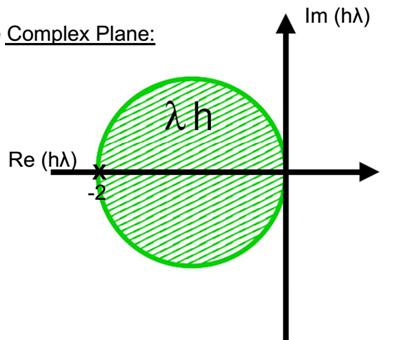
\includegraphics[width=.4\textwidth]{stab_euler_exp}\\
 \end{center}
 \caption{The stable region represented on the complex plane.} 
 \label{fig:stab_euler_exp}
\end{figure}

In general, we can treat $h \lambda$ together as a complex number, and the condition
$| 1 + h \lambda | \leq 1$ can be represented by a circle in the complex plane (Fig. \ref{fig:stab_euler_exp})
centered at $(-1, 0)$ with a radius of 1; \textbf{inside} this circle the solution is stable.
The implication is that for a given system (thus given $\lambda$), we have to choose the stepsize $h$ carefully
so that the Euler's method gives stable solution.

Now recall Example \ref{exmp:euler} where the Euler's method was used to solve $dx/dt=-0.5 x, x(0) = 100$.
Here $\lambda = -0.5$. To ensure stability, $| 1 - 0.5 h | \leq 1$, which means
\[  -1 \leq 1 - 0.5 h \leq 1 \]
\noindent which results in $ 0 \leq h \leq 4$. This is why when $h = 5$, the solution becomes unstable
as seen in Fig. \ref{fig:euler_stepsize}.

\end{exmp}


\begin{exmp}[Stability of the \textbf{implicit} Euler's method for solving linear ODEs]
Now consider using the implicit Euler's method to solve the same ODE, $d y / d t = \lambda y$ with initial condition $y(0) = y_0$, where
we progress from time point $n$ to $n+1$ ($h$ is the stepsize):
\[
	y_{n+1} = y_n + h f(y_{n+1}, t_{n+1}) = y_n + h \lambda y_{n+1}
\]
\noindent Solving the above for $y_{n+1}$, we have
\[
	y_{n+1} = (1 - h \lambda)^{-1} y_n
\]
\noindent Similarly we can obtain the following when progressing from time point $n-1$ to $n$:
$y_n = (1 - h \lambda )^{-1} y_{n-1}$, which when substituted into the above equation gives
\[
	y_{n+1} = (1 - h \lambda )^{-2} y_{n-1}
\]
\noindent Repeating this process recursively until we reach time point 0, we will get 
\[
	y_{n+1} = (1 - h \lambda )^{-(n+1)} y_0 =  \left( \frac{1}{1 - h \lambda} \right)^{n+1} y_0
\]

Therefore to ensure a stable solution using the implicit Euler's method, we must have
$ 1 / | 1 - h \lambda | \leq 1$ or equivalently $ | 1 - h \lambda | \geq 1$.
Similarly by treating $h \lambda$ together as a complex number, the condition
$| 1 - h \lambda | \geq 1$ can be represented by a circle in the complex plane (Fig. \ref{fig:stab_euler_imp})
centered at $(1, 0)$ with a radius of 1; \textbf{outside} this circle the solution is stable.

\begin{figure} [!h]
 \begin{center}
	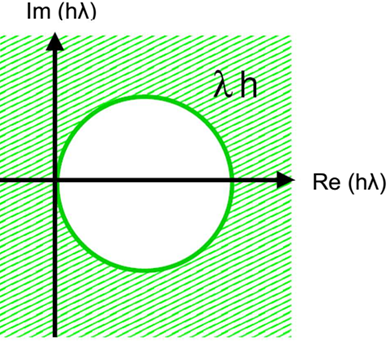
\includegraphics[width=.4\textwidth]{stab_euler_imp}\\
 \end{center}
 \caption{The stable region represented on the complex plane.} 
 \label{fig:stab_euler_imp}
\end{figure}

Now if we were to apply the implicit Euler's method to solve $dx/dt=-0.5 x, x(0) = 100$ in Example \ref{exmp:euler},
where $\lambda = -0.5$, stability is ensured if $| 1 + 0.5 h | \geq 1$, which means
\[  1 + 0.5 h \geq 1 \quad \textrm{or} \quad 1 + 0.5h \leq -1 \]
\noindent Since $h$ is the stepsize and must be positive, $1 + 0.5 h \geq 1$ always holds.
Therefore, regardless of the choice of stepsize, the implicit Euler's method will give a stable solution.

\end{exmp}

\textbf{In general}, implicit methods are more stable than their explicit counterparts, though they
usually involve more computation. In addition, for stiff problems implicit methods should be considered
as they allow much larger stepsize than explicit methods do, offering computational efficiency.
The latter point is further explored in tutorial sessions.

\subsubsection*{Global \& local errors of numerical solutions}

Error in a numerical solution refers to some kind of difference between the exact
solution and the numerical solution. No numerical method can completely avoid
error, but a good method should be able to contain the error within a certain limit.

\textbf{Global error.} This error refers to the difference between the exact solution and 
the numerical solution at a particular time point $t_n$. It contains errors accumulated from the previous steps 
as well as the local error introduced by the current time step.

\textbf{Local error.} At $t_n$, this error refers to the difference between 
(1) the exact solution of the original ODE with the numerical solution for $t_{n-1}$ as its initial condition, 
and (2) the numerical solution for $t_n$.

\begin{figure} [!h]
 \begin{center}
	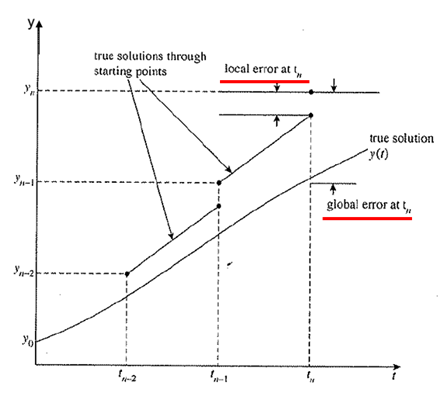
\includegraphics[width=.6\textwidth]{error}\\
 \end{center}
 \caption{Illustration of local and global errors in solving ODEs.} 
 \label{fig:error}
\end{figure}

The relationship between local and global errors is illustrated in Fig. \ref{fig:error}.
Usually, ODE solvers try to control the local error for computational efficiency, usually
by varying stepsizes. Here we use the RK methods to illustrate the idea of error control;
other algorithms follow similar principles.

The first step is to estimate the local errors; there are two approaches that can serve this purpose.
\begin{enumerate}
	\item \textbf{Extrapolation.} For integration from $t_{n-1}$ to $t_n$ thus stepsize is $h=t_n - t_{n-1}$, 
		the solution is calculated twice. The first with step size as $h$, and the second with two half-steps
		(i.e. from $t_{n-1}$ to $t_{n-1} + h/2$, and then from $t_{n-1} + h/2$ to $t_n$. By cutting the stepsize
		by half, the solution is generally more accurate. The difference of the two solutions is then used
		to estimate the local error of this step.
	\item \textbf{Embedding.} Two methods of different orders (thus different accuracy) are used to calculate
		the solution from $t_{n-1}$ to $t_n$, and the difference in solution is used as an estimate of the local error.
		This is a widely used technique in many numerical packages.
\end{enumerate}

Once the local errors are estimated, the stepsize for the next step $n+1$ can be adjusted by
\[ h_{n+1} = h_n \left( \frac{\tau}{E_n} \right)^{\frac{1}{p+1}} \]
\noindent where $\tau$ is the user-defined error tolerance (i.e. the maximum error allowed),
$E_n$ is the estimated local error, and $p$ is the order of the RK method.
Essentially, the formula increases the stepsize if $E_n < \tau$ (i.e. if the error is smaller than
the tolerance, we can afford to use a larger stepsize to save computation), and decreases the stepsize
if $E_n > \tau$ (i.e. if the error is greater than
the tolerance, we should use a smaller stepsize to improve accuracy).
In most ODE solver packages (e.g. Matlab's ODE solvers), similar method for stepsize adjustment is done
automatically.


\section{Differential-algebria equation (DAE) solution strategies}

As introduced in Lecture 4, the general form of a DAE system is
\begin{align}
	\frac{d x}{d t} = f(x, y, t) \quad &\leftarrow \quad \textrm{ODEs} \\
	g(x, y, t) = 0 \quad &\leftarrow \quad \textrm{Algebraic equations} \\
	x(0) = x_0  \quad &\leftarrow \quad \textrm{Initial conditions}
\end{align}
\noindent where $x$ is a set of differential variables and $y$ a set of algeraic variables.

Here we use an example to explain the three methods for solving DAE systems.

\begin{exmp}[Modelling tank level]
Shown in Fig. \ref{fig:tank} is an example we discussed in Lecture 4. Here
we quote the modelling equations which are in the form of a DAE system:

\begin{align}
	\frac{d h}{d t} &= \frac{1}{A} ( F_1 - F_2 ) \label{eq:tank1} \\
	F_1 - & C_V \sqrt{P_1 - P_2} = 0 \label{eq:tank2} \\
	F_2 - & C_V \sqrt{P_2 - P_3} = 0 \label{eq:tank3} \\
	P_2 - & P_0 - \rho g h = 0 \label{eq:tank4}
\end{align}
\noindent where $P_1$ and $P_3$ are measured and thus known;
in addition, $\rho$, $A$ and $g$ are constants and thus also known.
The initial condition is specified: $h(t=t_0) = h_0$.

\begin{figure} [!h]
 \begin{center}
	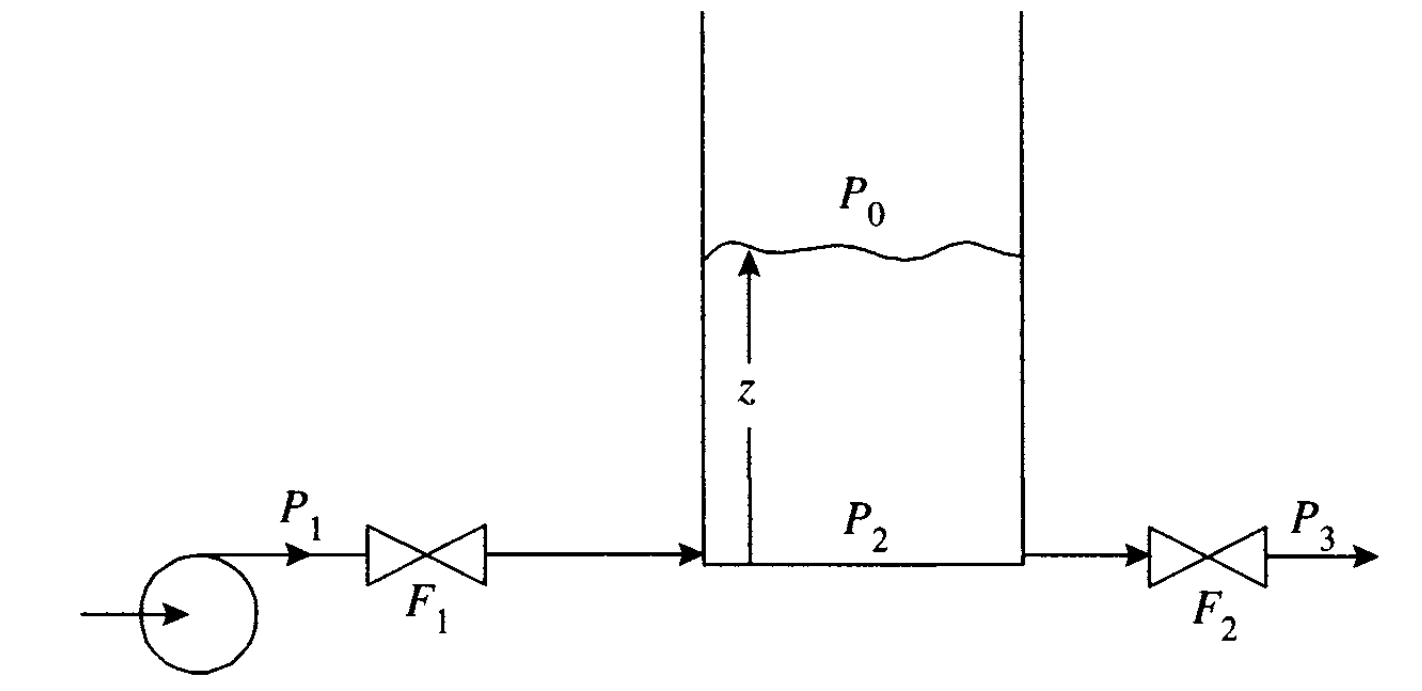
\includegraphics[width=.6\textwidth]{tank}\\
 \end{center}
 \caption{A tank system modelled by DAEs.} 
 \label{fig:tank}
\end{figure}

\begin{itemize}
	\item \underline{Method 1: Substitute for algebraic variables to convert DAE to ODE.}\\
		From eq. (\ref{eq:tank4}) we obtain $P_2 = P_0 - \rho g h$ which can be
		substituted into eqs. (\ref{eq:tank2})(\ref{eq:tank3}) to get
		\[ F_1 = C_V \sqrt{P_1 - P_0 - \rho g h} \]
		\[ F_2 = C_V \sqrt{P_0 + \rho g h - P_3} \]
		which then can be substituted into eq. (\ref{eq:tank1}) to result in the final ODE:
		\begin{equation}
			\frac{d h}{d t} = \frac{1}{A} \left[ C_V \sqrt{P_1 - P_0 - \rho g h} - C_V \sqrt{P_0 + \rho g h - P_3} \right]
		\end{equation}
	\item \underline{Method 2: Solve the ODEs and algebraic equations separately.} \\
		Starting from the initial time $t_0$ with specified initial condition $h_0$,
		solve eqs. (\ref{eq:tank2})(\ref{eq:tank3})(\ref{eq:tank4}) using an algebraic solver
			(discussed in Section \ref{sec:alg}) to obtain the value of $F_1$, $F_2$ and $P_2$
			at time $t_0$. Then use an explicit ODE solver to solve eq. (\ref{eq:tank1}) from $t_0$ to $t_1$, where
			the right-hand side of eq. (\ref{eq:tank1})
			requires the value of $F_1$ and $F_2$ as obtained by the algebraic solver.
			Repeat this process from $t_1$ to $t_2$, and so on.
	\item \underline{Method 3: Solve the ODEs and algebraic equations simultaneously.} \\
		Use an implicit ODE solver to convert eq. (\ref{eq:tank1}) into an algebraic equation from $t_0$ to $t_1$,
		which is combined with eqs. (\ref{eq:tank2})(\ref{eq:tank3})(\ref{eq:tank4})
		to form a combined set of algeraic equations. Then solve this set of equations using an algebraic equation
		solver to obtain the value of $h$, $F_1$, $F_2$ and $P_2$ at $t_1$. Repeat this process from
		$t_1$ to $t_2$, and so on.
\end{itemize}

Although Method 1, the direct substitution method, seems the most attractive, it is only possible when
we can analytically solve eqs. (\ref{eq:tank2})(\ref{eq:tank3})(\ref{eq:tank4}). Method 2, as an explicit
method, is not suitable for stiff problem. Method 2 is also computationally slow because of the need to
solve the algebraic equations repeated whenever we need to solve the ODE, where a lot of such calculations
are needed in multi-step and/or multi-stage ODE solvers (e.g. the RK and BDF methods).
Therefore, Method is the most frequently used in many numerical DAE solvers.

\end{exmp}

\begin{thebibliography}{3}
\vspace{-0.4cm}
\bibitem[{Brenan(1989)}]{Brenan1989}
Brenan KE, Campbell SL, Petzold LR, 1989. Numerical solution of Initial-value problems in differential-algebraic equations. North-Holland.

\bibitem[{Hangos(2001)}]{Hangos2001}
	Hangos KM, Cameron IT, 2001. Process Modelling and Model Analysis, Academic Press: London.

\bibitem[{Shampine(1997)}]{Shampine1997}
Shampine LF, Reichelt MW, 1997. The MATLAB ODE Suite, SIAM Journal on Scientific Computing, 18: 1–22.

\end{thebibliography}

\end{document}


